\section{Руководство по пересборке ОРП}
%\marginnote{\Date{Чт.}{19}{Июл.}{2018}}[-40pt]

\begin{itemize}	
	\item Открываем обработку <<Открыть редактирования чеков ККМ>>  - \menu[,]{Продажи, Дополнительные обработки, }
	
	
	\begin{figure}[H]
		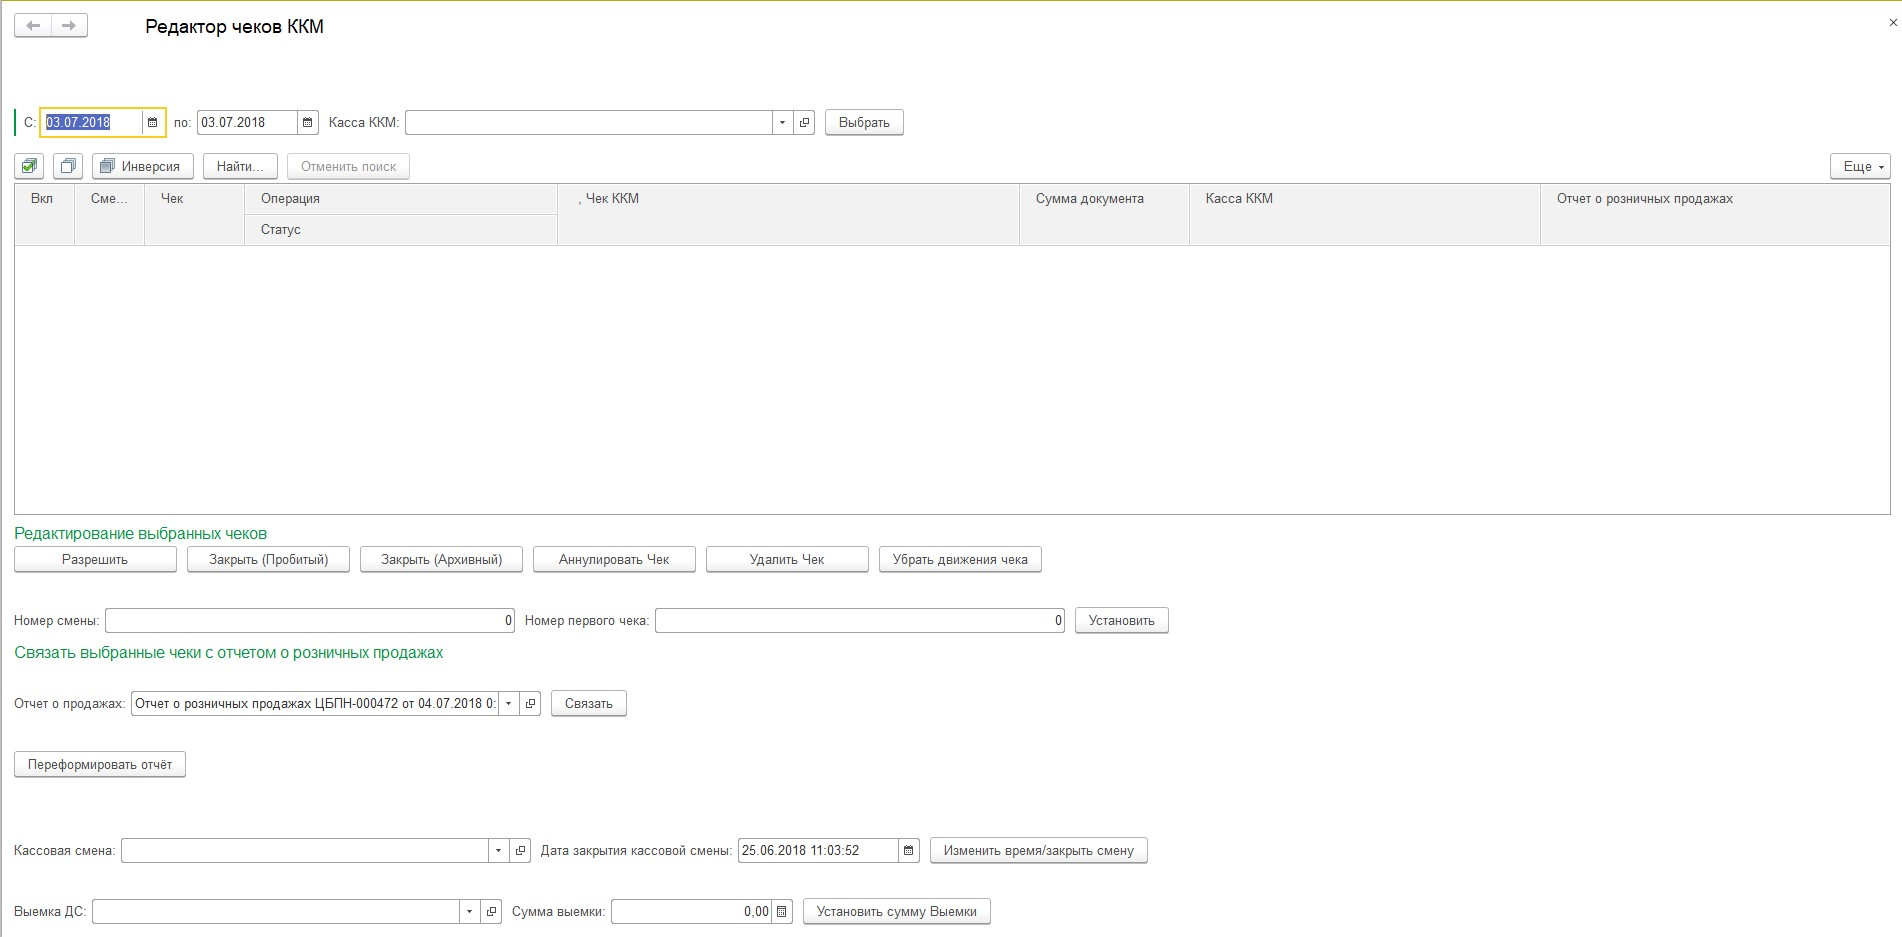
\includegraphics[width=0.7\textwidth]{18.jpg}
		\caption{<<Редактирование чеков ККМ>>.}
		\label{ris:18.jpg}
	\end{figure}

	\item Далее выполняем следующие действия:
	
	\begin{enumerate}[label={\alph*)},font={\color{red!50!black}\bfseries}] 
		
		\item Устанавливаем период, в котором находится интересующий нас чек и кассу ККМ. Нажимаем кнопку \keys{Выбрать}.
		
		\begin{figure}[H]
			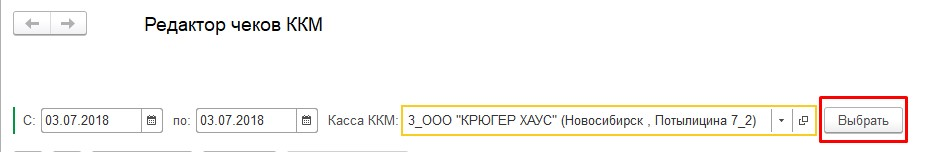
\includegraphics[width=1.0\textwidth]{19.jpg}
			\caption{<<Настройка отбора>>.}
			\label{ris:19.jpg}
		\end{figure}
		
		Табличная часть заполняется чеками за период по выбранной кассе.
		
		\item Выделяем мышкой колонку, по которой будем производить поиск нужного чека. В нашем случае это <<Сумма документа>>. Нажимаем кнопку \keys{Найти}.
		
		\begin{figure}[H]
			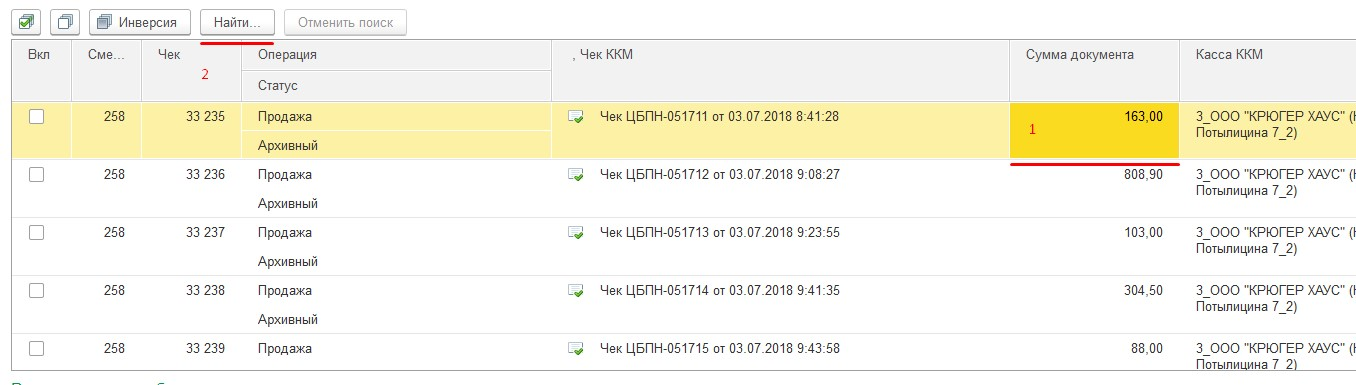
\includegraphics[width=1.0\textwidth]{20.jpg}
			\caption{<<Поиск чека>>.}
			\label{ris:20.jpg}
		\end{figure}
	
		Во всплывающем окошке указываем сумму искомого чека. Нажимаем кнопку \keys{Найти}.	
		
		\begin{figure}[H]
			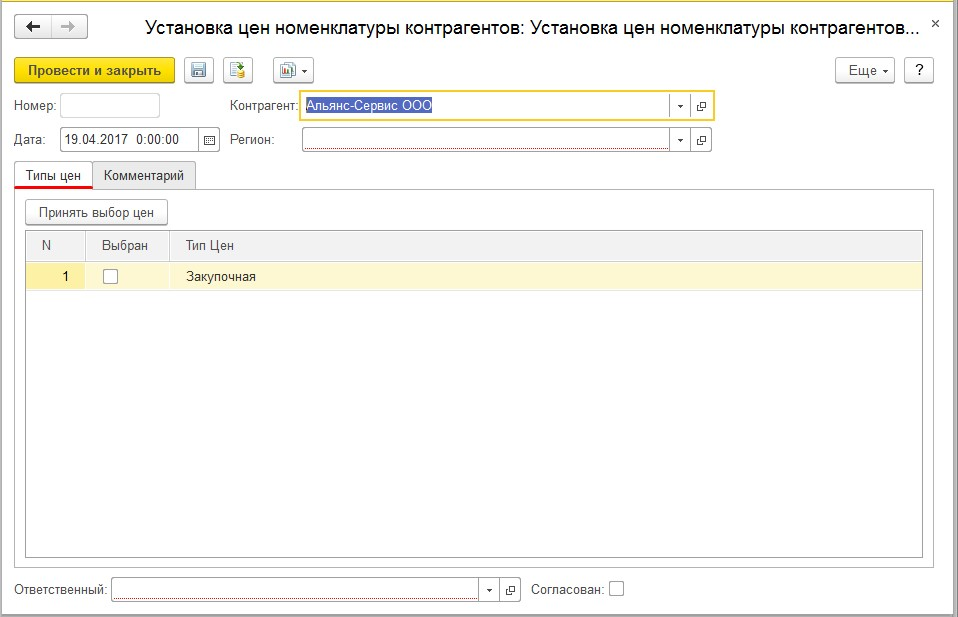
\includegraphics[width=0.5\textwidth]{21.jpg}
			\caption{<<Окно поиска>>.}
			\label{ris:21.jpg}
		\end{figure}
		
		Чек найден. (Рис.~\ref{ris:22.jpg})
		
		\begin{figure}[H]
			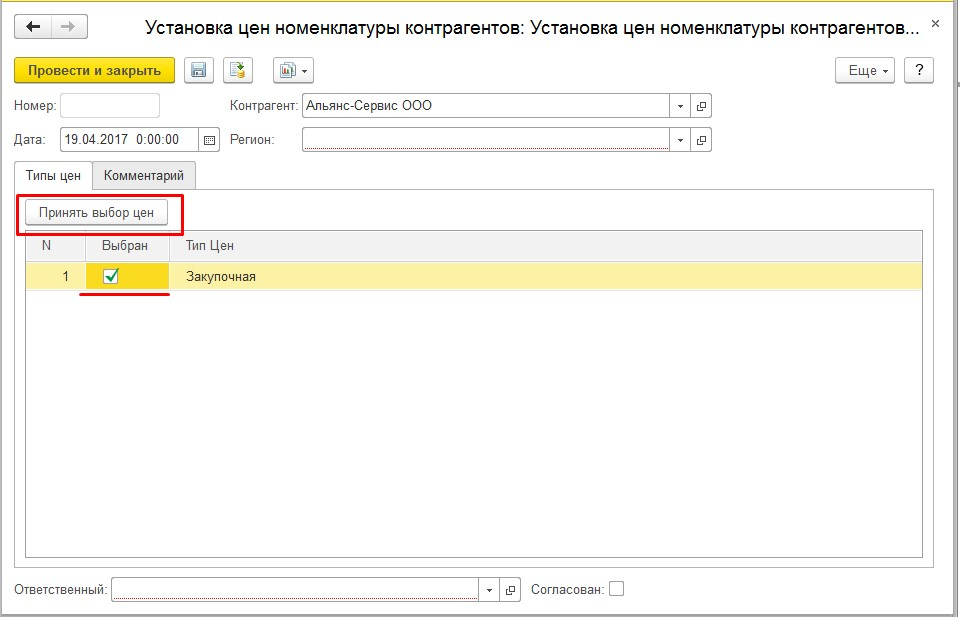
\includegraphics[width=0.9\textwidth]{22.jpg}
			\caption{<<Найденный чек>>.}
			\label{ris:22.jpg}
		\end{figure}
		
		\item Отмечаем чек. \par Далее последовательно нажимаем кнопки \keys{Разрешить}, \keys{Закрыть (Пробитый)}, \keys{Закрыть (Архивный)} 
		Каждый раз после нажатия кнопки  восстанавливая отметку чека.
		
		\begin{figure}[H]
			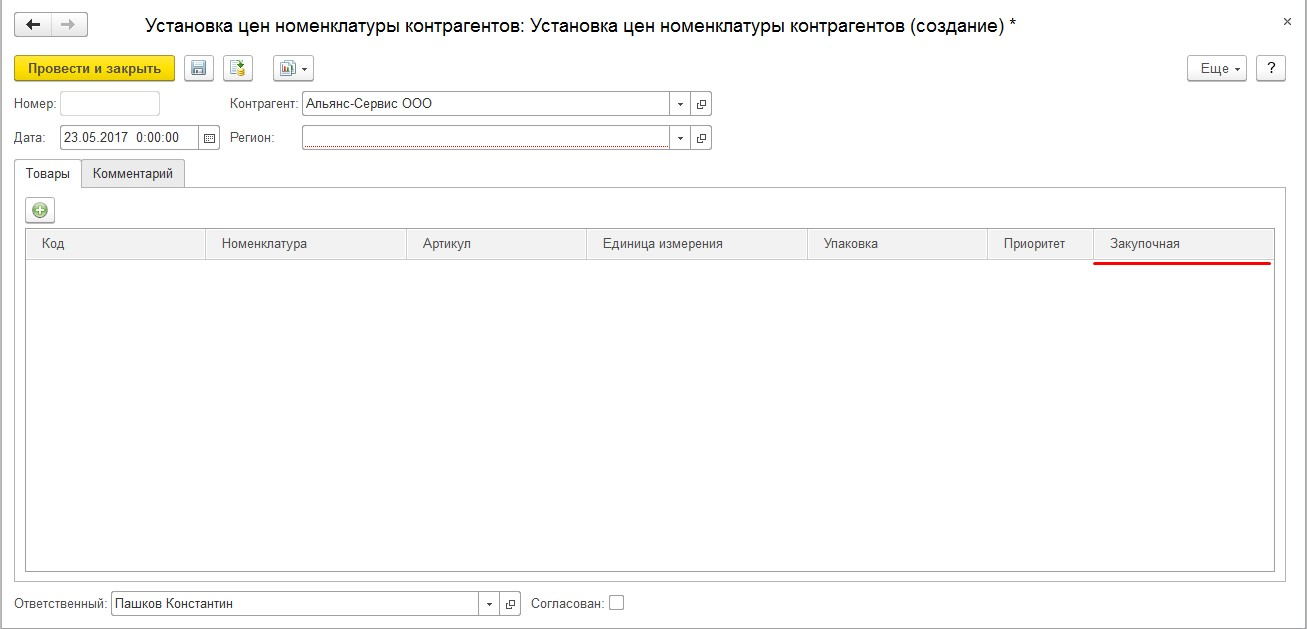
\includegraphics[width=0.9\textwidth]{23.jpg}
			\caption{<<Работа с чеком>>.}
			\label{ris:23.jpg}
		\end{figure}

		После всех операций чек принимает статус <<Архивный>> (Рис.~\ref{ris:24.jpg})

		\begin{figure}[H]
			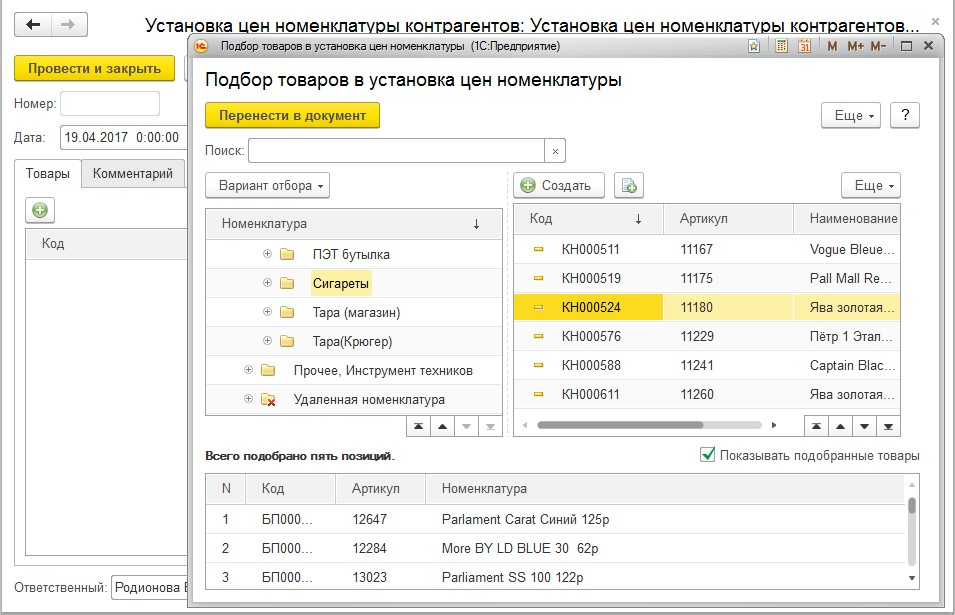
\includegraphics[width=0.9\textwidth]{24.jpg}
			\caption{<<Статус чека>>.}
			\label{ris:24.jpg}
		\end{figure}
		
		
		\item Указываем отчет о розничных продажах с которым планируем связать чек. Проверяем, что отметка на чеке стоит, нажимаем кнопку  \keys{Связать}
		
		\begin{figure}[H]
			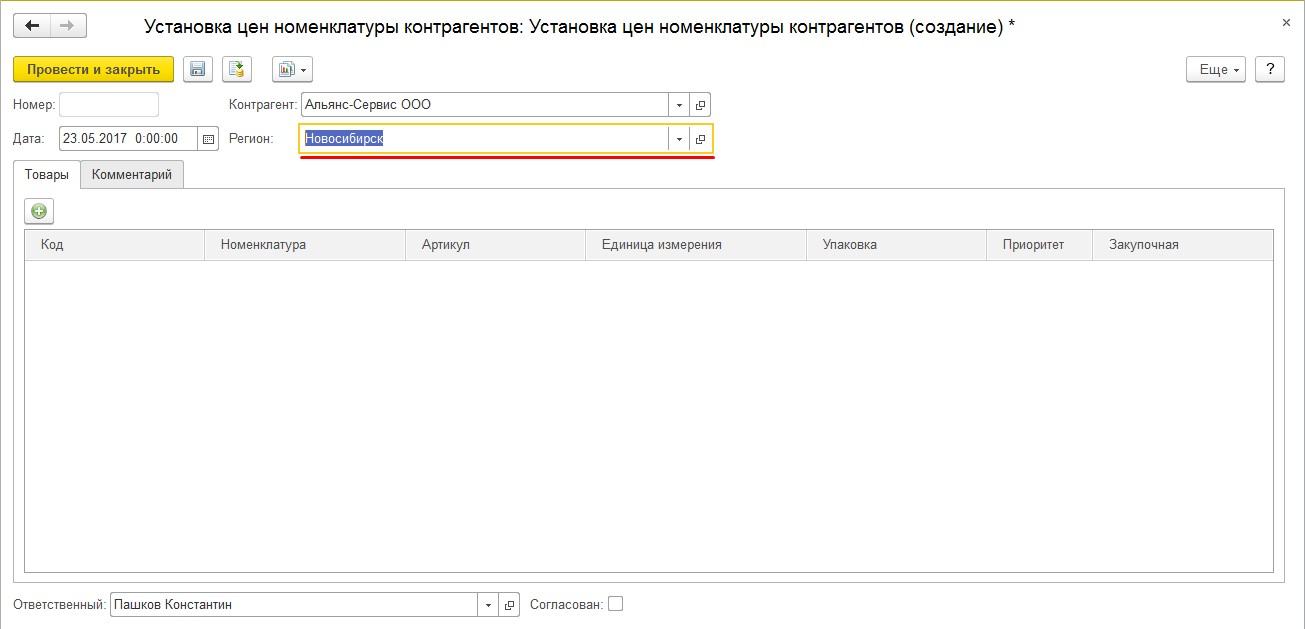
\includegraphics[width=0.9\textwidth]{25.jpg}
			\caption{<<ОРП>>.}
			\label{ris:25.jpg}
		\end{figure}
	
		После выполнения нажимаем кнопку \keys{Переформировать отчет}
		
	\end{enumerate}	
	
	\item Отчет сформирован. Переходим в ОРП на вкладку <<Дополнительно>> и  при редактировании данных нажимаем кнопку  \keys{Пересчитать}
		
		\begin{figure}[H]
			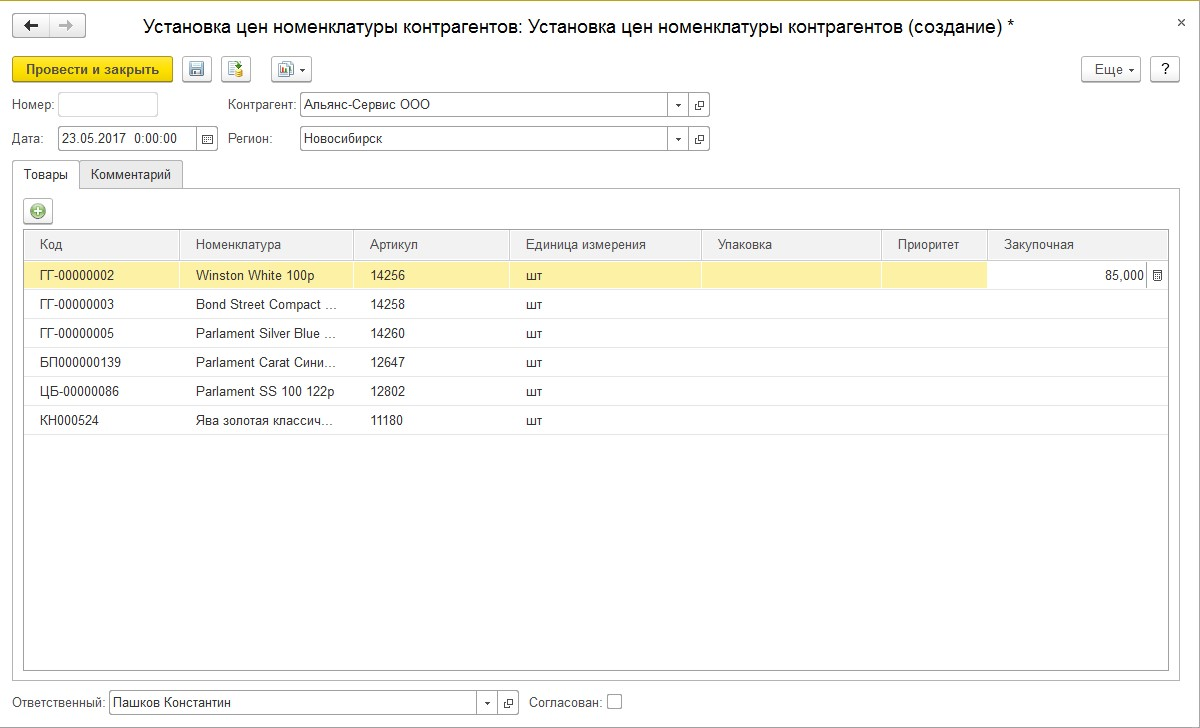
\includegraphics[width=0.5\textwidth]{26.jpg}
			\caption{<<Корректировка>>.}
			\label{ris:26.jpg}
		\end{figure}
	
\end{itemize}
